\documentclass[a4paper,12pt]{report}


\usepackage[english]{babel}
\usepackage[T1]{fontenc}
\usepackage[toc,page]{appendix}
\usepackage{amssymb}
\usepackage{amsmath}
\usepackage{latexsym}
\usepackage{physics}
\usepackage{listings}
\usepackage{graphicx}


\begin{document}{\textbf{MAPD FPGA Lab 5 - Homework Report - Vincenzo Maria Schimmenti 1204565}}\\
This homework is about implementing in VHDL a finite impulse response (FIR) filter. A FIR filter is a digital filter characterized by a finite duration impulse response, i.e. calling
$c[n]$ the impulse response we would have:
$$c[n]=\begin{cases}
\neq 0 & 0 \leq n \leq N \\
= 0 & \textrm{otherwise}
\end{cases}$$
Given a signal $x[n]$ the output signal $y$ is the convolution:
$$y[n+1]=c \circledast x = \sum_{i=0}^{n} c[i]x[n-i]$$
Our version of the filter employs a filter with five terms:\\
\begin{figure}[h!]
	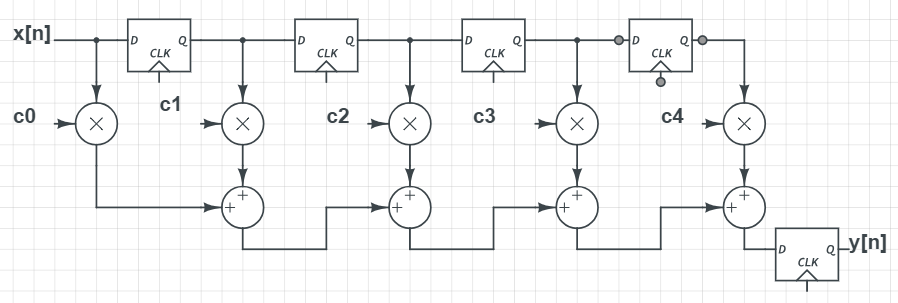
\includegraphics[width=\linewidth]{fir5.png}
	\caption{A 5-tap FIR}
	\label{fig:fir5}
\end{figure}\\
Since the duration of the filter is 5 we need to employ, at each instant $n$, 4 flip-flops to store the previous 4 values of $x$ and another flip-flop to store the output:
$$y[n+1]=c_0 x[n] + c_1x[n-1]+c_2x[n-2]+c_3x[n-3] + c_4x[n-4]$$
At time $n=0$ all the flip-flops are set to $0$ (thanks to a reset signal). The system is driven by a clock signal that, going from 0 to 1, triggers the flip flops: at instant $n$, in a parallel fashion, the first flip-flop stores the old input $x[n-1]$ while the other 3 store their left flip flop value. The last flip flop stores the convolution result and is as well updated by the clock signal.
\newpage
For example for $c[0]=1 \quad c[1]=2 \quad c[2]=3 \quad c[3]=4 \quad c[4]=5$ and $x[n]=1 \quad \forall n$ we would get $y[0]=0\quad y[1]=1 \quad y[2] =3 \quad y[3] = 6 \quad y[4] = 10 \quad y[5]=15$. The simulation on Vivado gives:
\begin{figure}[h!]
	\begin{center}
		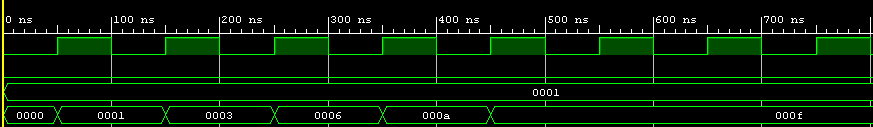
\includegraphics[width=1.2\textwidth,keepaspectratio]{fir5ex.png}
	\end{center}	
	\caption{A 5-tap FIR example}
	\label{fig:fir5ex}
\end{figure}\\
The first row is the clock, the second is the reset signal, the third is the input and the last is the output.\\
The testbench uses one component, the fir filter component,
which itself uses the flip flop component. All the inputs and output are logic vectors of length $N=16$ and the operations (addition and multiplication) are done via signed type numbers, either of length 16 or 32. The fir filter entity reads the value from flip flops as logic vectors, converts them into signed, does the convolution then performs the right shift of $Q=11$ bits and takes (since the result of the operation is 32 bits long) the lower 15 bits and the leading sign. The shift is needed since the coefficents of the filter are supposed to be premultiplied (i.e. left shifted) by $2^{11}$; we can see that for the coefficents we used a fixed point representation with 1 bit for the sign, 4 bits for the integer part and 11 for the fractional part; for example the number $0.19335315$ is in binary represented (approximately) by $0.00110001011$ so the sign bit is $0$ the integer part is $0000$ and the fractional is $00110001011$ so in hexadecimal the number is represented by 0x18B.
\end{document}